\section{Sacred Science 104: Essence and Substance}

Purusha and prakriti are the two poles of all manifestation.

\textbf{Purusha} is the active principle, represented as masculine.

\textbf{Prakriti} is the undifferentiated primordial substance. It is the passive principle, represented as feminine. It is purely potential and passive, capable of any determination while actually possessing none. Prakriti therefore cannot be a cause by itself (i.e., efficient cause), apart from the action or rather the influence of the essential principle, which is Purusha, and which is the determinant of manifestation.

Universal Being is one, and is polarized. All manifested things are produced by Prakriti, of which they are modifications or determinations. But without the presence of Purusha, these productions would be devoid of all reality. In other words, the productions would be nothing in particular, but rather random variations of the Purusha.

\begin{wrapfigure}{ht}{0.35\textwidth}
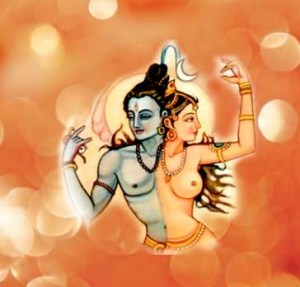
\includegraphics[scale=.4]{a20221006SacredScience104EssenceandSubstance-img001.jpg} 
\end{wrapfigure}

In the West, this teaching is called hylomorphism and has gone by names like “form and matter” or, in Greek, eidos and hyle. Guenon prefers the terms “essence” and “substance”, because if taken in their broadest sense, they provide the most exact idea of the conception in Western languages.

\paragraph{Productions of Prakriti}
Purusha is neither productive nor a production. Nevertheless, Its action essentially determines everything that is substantial production in Prakriti. However, this action is “nonacting activity”.

Prakriti is also not a production, but it is productive. There are seven principles, or productions of Prakriti that give rise to manifestation. These are:

\begin{enumerate}
\item \textbf{Buddhi}. This is the Higher Intellect, which is formless manifestation. Thus, Intelligence is at the beginning of manifestation, so it does not arise randomly from something lower. 
\item \textbf{Ahankara}. This is the ego or individual consciousness brought about by thought. It is the reflection of Buddhi in subtle manifestation. 
\item \textbf{Tanmatras}. These are the essential determinations of things, which are incorporeal and outwardly imperceptible as they are part of subtle manifestation. These include the senses of hearing, touch, sight, taste, and smell. Hence, the possibilities of sensual awareness is prior 
\item \textbf{Manas}. The Mind includes mental functions related to thinking, such as memory, imagination, and common sense. 
\item \textbf{Buddhindriyas}. These are the faculties of sensation associated with the respective tanmatra. As such, they bridge the subtle and gross states. The ear, skin, eyes, tongue, and nose are produced in order to experience the tanmatras. 
\item \textbf{Karmendriyas}. These are the faculties of action such as locomotion, manipulation, reproduction, elimination, and speech. The need for such faculties forms the body. 
\item \textbf{Bhutas}. These are the five substantial and sensible elements which form gross manifestation 
\end{enumerate}
\paragraph{The Three Forces}
Purusha is the ordering principle for Prakriti. There are three forces, called gunas, in Prakriti which are in perfect balance in its primordial state. However, beings, in their various states, relate to these forces in different degrees. These are the three gunas, along with their names in the Western tradition.

\begin{itemize}
\item \textbf{Sattva or Neutralizing Force}: conformity to the pure essence of Being (Sat), which is identified with intelligible Light or Knowledge, and represented as an ascending tendency. 
\item \textbf{Rajas or Positive Force}: the expansive impulse, according to which the being develops in a certain state and, in some way, at a determined level of existence. 
\item \textbf{Tamas or Negative Force}: darkness, equated with ignorance, and represented as a downward tendency. 
\end{itemize}
Beings must strive to keep these forces in balance.

\paragraph{The Human State}
When it comes to the corporeal body in the human state, then matter is, in some way, analogous to Prakriti. We certainly don't count on science to prove anything, but it is appropriate to point out that science is consistent with metaphysics. Here are two major points.

\textbf{Matter is indeterminate}. According to quantum theory, matter is fundamentally indeterminate, being nothing more than probability waves. A thing comes into existence through a collapse of the wave function; how that happens is unknown and is called the “measurement problem”. The Traditional teaching is that a higher intelligence, through non-acting acting, instigates the Purusha to produce forms.

\textbf{Matter has no qualities}. Science advanced when it removed all qualia from its observations. Hence, qualia like color, taste, odor, and sound have no place in science and are not part of any equation. Traditional teaching agrees with this; i.e., the sense arise in consciousness, not in matter. Human consciousness, therefore, participates in the creation of the world by adding sense and intelligibility to it.

Biology today assumes that the organs of sense and action arose accidently through random variations. But why would sense organs arise, and what survival value can they provide, if matter is devoid of qualities? Why would analogous organs of action arise randomly? Traditional teaching is opposite to that, since it teaches that these organs are the result of will. In this extract, Valentin Tomberg summarizes those teachings; those of you on the fence can decide which version sounds more plausible.

\begin{quotationx}
Tentacles, paws, arms, wings — are they not simply diverse forms manifesting a common prototype or principle? They are in so far as they express the desire to bear the sense of touch further, to be able to touch things more removed than those in the immediate neighborhood of the surface of the body. They are active extensions of the passive and receptive sense of touch which is spread out over the surface of the organism. In making use of them, the sense of touch makes “excursions” from its usual orbit circumscribed by the skin which covers the body.

The organs of action are simply crystallized will. I walk not because I have legs but rather, I have legs because I have the will to move about. I touch, I take and I give not because I have arms, but I have arms because I have the will to touch, to take and to give. The “what” of the will engenders the “how” of the action (the organ), and not inversely. The arms are therefore the expression of the will to bear touch further than the surface of one's own body. They are the manifestation of extended touch, due to the will to touch things at a distance. It is similar with wings. They are also an exteriorised will — a will become organ.

\end{quotationx}

\textit{Image courtesy of Hindu website\footnote{\url{https://www.hinduwebsite.com/symbolism/purusha-prakriti-symbolism.asp}}}

\flrightit{Posted on 2022-10-06 by Cologero}